\documentclass[13pt]{beamer}
\usepackage{graphicx}
\usepackage[utf8]{inputenc}
\usepackage[skip=2pt,font=scriptsize]{caption}
\usepackage{algorithm}
\usepackage{algorithmic}

% Algorithms
\renewcommand{\algorithmicrequire}{\textbf{Summary:}}
\renewcommand{\algorithmicensure}{\textbf{Output:}}
\algsetup{linenosize=\small}

% Captions
\captionsetup{labelformat=empty,labelsep=none}
\DeclareCaptionFormat{myformat}{#3}
\captionsetup[algorithm]{format=myformat}

% References
\usepackage{url}
\bibliographystyle{acm}

\setbeamertemplate{bibliography item}[triangle]

% Formatting
\usetheme{Singapore}
\usecolortheme{whale}

% Title Page
\title{The Sieve of Eratosthenes using MPI}
\author{Devin Delfino}
\institute{Comp 401: Senior Seminar}
\date{4/16/2015}

% Table of Contents
\setbeamertemplate{section in toc}[sections numbered]
\setbeamercolor{alerted text}{fg=blue}
\AtBeginSection[]
{
  \begin{frame}
    \frametitle{Outline}
    \tableofcontents[currentsection]
  \end{frame}
}

\begin{document}
% TITLE ------------------------------------------------
\frame{\titlepage}


% Table of Contents ------------------------------------------------
\begin{frame}
\frametitle{Outline}
\tableofcontents
\end{frame}

\section{Parallel Programming and MPI} % ==========================================================================
% Parallel Programming Introduction ------------------------------------------------
\begin{frame}
\frametitle{Introduction}

\begin{itemize}
  \item \alert{Parallel Computing} is the use of multiple computers or processors to reduce the time needed to solve a single computational problem.
  \item A \alert{task} is a single program including local memory and a collection of input/output ports.
  \item A \alert{channel} is a message queue between two tasks used for communication
\end{itemize}
\end{frame}
% share definitions and talk about analogy
% workers = processors, job = program, tasks = tasks
% sequential -> assign the entire job to one person
% parallel -> divide the job into various tasks, assign the t tasks to p workers (maximize efficiency when t = p)
%          -> communication may be needed between the workers, representing comm. channels

% Foster's Design: Partitioning ------------------------------------------------
\begin{frame}
\frametitle{Ian Foster's Design Methodology}
  \begin{enumerate}
    \item \alert{Partitioning} - the process of dividing the computations and data into pieces.
    \item \alert{Communication} - channels between tasks allow communication between them
          \begin{itemize}
            \item Local - a task's computation requires values from a small number of other tasks
            \item Global - many tasks must contribute values to perform a computation
          \end{itemize}
    \item \alert{Agglomeration} - grouping tasks in order to improve performance and reduce overhead.
    \item \alert{Mapping} - assigning processes or tasks to specific processors or computers
  \end{enumerate}
\end{frame}
% partitioning - dividing computations into tasks domain vs functional decomp (divide data vs divide computations)
% communication - local means a task is dependent on data from a different task, global for example summing up a value from each task
% agglomeration - (not the focus) dividing computations into tasks to assign to varous processors
% mapping - (not the focus) 

% MPI Introduction ------------------------------------------------
\begin{frame}
\frametitle{Message Passing Interface (MPI)}
\begin{itemize}
  \item The most popular message-passing library standard % talk about the lack of portability/compatibility across computers
  \item There are many free implementations of MPI libraries, including OpenMPI and MPICH
  \item Integrates sequential language with functions that allow processes to communicate with each other
\end{itemize}
\end{frame}

\section{The Sequential Algorithm} % ==========================================================================
% The Sequential Sieve ------------------------------------------------
\begin{frame}
\frametitle{The Sequential Algorithm}
  \begin{algorithm}[H]
        \caption{The Sieve of Eratosthenes}
        \begin{algorithmic}
          \REQUIRE Finds all primes between $2$ and $n$, inclusive
          \STATE 1. Create a list of natural numbers $2$, $3$, ... , $n$, none of which are marked
          \STATE 2. Set $k$ equal to the first prime number, $2$
          \WHILE{$k^2 \leq n$}
            \STATE 3a. Mark all multiples of $k$ between $k^2$ and $n$
            \STATE 3b. Set $k$ to the smallest unmarked number greater than the current $k$
          \ENDWHILE
        \end{algorithmic}
        \end{algorithm}
\end{frame}
% Introduce steps
% SHOW ANIMATION

\section{The Parallel Algorithm} % ==========================================================================
% Block Allocation ------------------------------------------------
% \begin{frame}
% \frametitle{The Parallel Algorithm: Data Decomposition}
%   \begin{itemize}
%     % \item \alert{Decomposition} is the result of partitioning, agglomeration, and mapping
%     \item Partitioning - Breaking the array into pieces
%     \item Agglomeration - 
%   \end{itemize}
% \end{frame}

% Block Allocation ------------------------------------------------
\begin{frame}
\frametitle{The Parallel Algorithm: Block Decomposition}
  \begin{itemize}
    % \item \alert{Decomposition} is the result of partitioning, agglomeration, and mapping
    \item $n$ is the size of array and $p$ is the number of processors
    \item Divide the array into $p$ contiguous blocks of roughly equal size
    \item If $n$ is divisible by $p$, then there will be $p$ blocks of size $n / p$. Otherwise, there will be $p$ blocks of with sizes of either $\lfloor n / p \rfloor$ or $\lceil n / p \rceil$.
    \item Common data block computations include finding the first/last element controlled by a given process
  \end{itemize}
\end{frame}

\begin{frame}
\frametitle{The Parallel Algorithm: Block Decomposition, cont.}
  \begin{itemize}
    \item Suppose $n$ is the size of array and $p$ is the number of processors
    \item First element controlled by process $i$: $$\lfloor i n / p \rfloor$$
    \item Last element controlled by process $i$: $$\lfloor (i + 1) n / p \rfloor - 1$$
  \end{itemize}
\end{frame}

\begin{frame}
\frametitle{Block Decomposition Example, $n = 121$, $p = 3$}
    \alert{Processor 0:}
    \begin{itemize}
    \item First index: $\lfloor (0) (121) / 3 \rfloor = 0$
    \item Last index: $\lfloor (0 + 1) 121 / 3 \rfloor - 1 = \lfloor 40\frac{1}{3} \rfloor - 1 = 39$
    \item Size: $\text{last - first + 1} = \lfloor n / p \rfloor = 40$.
    \end{itemize}

    \alert{Processor 1:}
    \begin{itemize}
    \item First index: $\lfloor (1) (121) / 3 \rfloor = \lfloor 40\frac{1}{3} \rfloor = 40$
    \item Last index: $\lfloor (1 + 1) 121 / 3 \rfloor - 1 = \lfloor 80\frac{2}{3} \rfloor - 1 = 79$
    \item Size: $\text{last - first + 1} = 40 = \lfloor n / p \rfloor$.
    \end{itemize}

    \alert{Processor 2:}
    \begin{itemize}
    \item First index: $\lfloor (2) (121) / 3 \rfloor = \lfloor 80\frac{2}{3} \rfloor = 80$
    \item Last index: $\lfloor (2 + 1) 121 / 3 \rfloor - 1 = \lfloor 121 \rfloor - 1 = 120$
    \item Size: $\text{last - first + 1} = 41 = \lceil n / p \rceil$.
    \end{itemize}

\end{frame}

% Translating Sequential Algorithm 1------------------------------------------------
\begin{frame}
\frametitle{Developing the Algorithm, Step 1}
\alert{1. Create a list of natural numbers $2$, $3$, ... , $n$, none of which are marked}
\begin{itemize}
  \item Each task handles a specific block of the entire array
  % \item Use the formulas to determine the numbers represented by the first and last elements of the block along with its size
  \item To minimize communication between tasks, make task 0 responsible for finding the next value of $k$
  \item This can be done by ensuring $n/p > \sqrt{n}$
  \item Keep in mind the difference between the local index for the block and the global index for the entire array
\end{itemize}
\end{frame}

% Translating Sequential Algorithm 2------------------------------------------------
\begin{frame}
  \alert{2. Set $k$ equal to the first prime number, $2$}
  \begin{itemize}
    \item $k$ is set to the first prime number for all tasks
    \item After each iteration, each task must be told the next value of $k$

  \end{itemize}
\end{frame}

% Translating Sequential Algorithm 3------------------------------------------------
\begin{frame}
\frametitle{Developing the Algorithm, Step 3}
\alert{While $k^2 \leq n$\\}
\alert{3a. Mark all multiples of $k$ between $k^2$ and $n$}
\begin{itemize}
  \item Must determine the first multiple of $k$ in the given block (if it's greater than $k^2$)
  \item From the first multiple of $k$, mark every $k^{th}$ element
\end{itemize}

\alert{3b. Set $k$ to the smallest unmarked number greater than the current $k$}
\begin{itemize}
  \item The smallest unmarked number greater than the current $k$ is always part of the block belonging to task 0
  \item Task 0 finds the next value of $k$, and broadcasts it to the rest of the tasks
\end{itemize}
\end{frame}

\section{Sequential vs. Parallel Comparison} % ========================================================================
% Comparison: Seq vs. Par ------------------------------------------------
\begin{frame}
\frametitle{Sequential vs. Parallel}
  \begin{figure}
    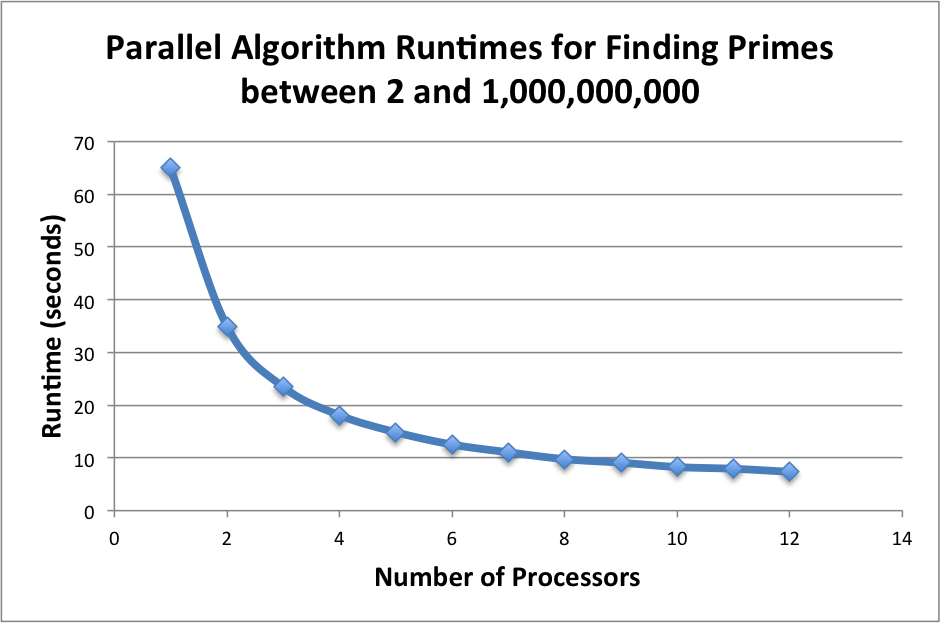
\includegraphics[height=7cm]{./sieve_benchmark.png}
  \end{figure}
\end{frame}

% References ------------------------------------------------
 \begin{frame}
  \frametitle{References}
  \nocite{*} 
  \bibliography{workscited}
\end{frame}

\end{document}